\chapter{Laozi et le Daode jing}

\subsection{Laozi}
\paragraph{Disparate et complexe}

\paragraph{Laozi, personnage légendaire} Cité dans un ouvrage du IV av JC. Au II av JC, la première biographie. 



Laozi, un personnage largement légendaire


Éléments principaux de la légende concernant Laozi:
\begin{itemize}
    \item  	Il aurait eu pour nom Li, pour prénom Er
    \item 	Il aurait été archiviste ou annaliste-devin de la dynastie Zhou
    \item 	La visite que Confucius lui aurait rendue
    \item 	Son exil vers l’ouest à dos de buffle
    \item 	A 50 ans, il arrive sur un buffle noir. Le gardien est content. Il demande à Laozi de coucher son enseignement. Sa rencontre avec Yin Xi, le gardien de la passe, qui lui demanda de coucher par écrit sa doctrine, le classique de le \textit{voie et de la vertu}
\end{itemize}




\begin{marginfigure}
    \centering
        \caption{Laozi sur le buffle Zhang Lu (1490-1563)}
    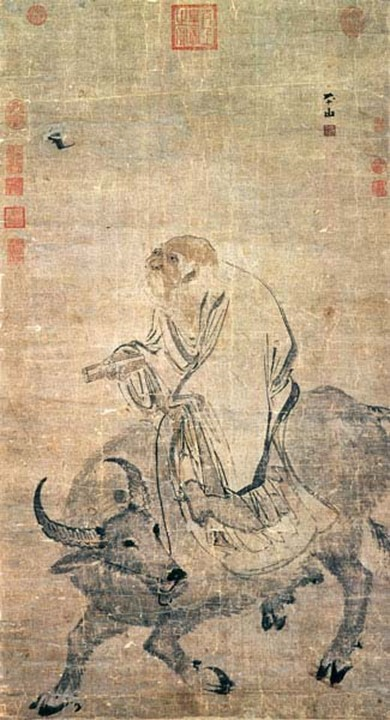
\includegraphics[width=\textwidth]{ConfucianismeTaoismeBouddhismeChinois/Images/Laozi.jpg}

    \label{fig:enter-label}
\end{marginfigure}



\paragraph{L'Ouest} Théorie qui arrive au IIè siècle selon lequel il voulait aller en Inde devenir un Bouddha.



 \subsection{Le Laozi ou le Daode jing }

\paragraph{81 chapitres courts en deux parties} 
une première partie, \textit{classique du Dao / voie} et une deuxième partie, \textit{classique} (jing) de la vertu (\textit{de}). l'ensemble s'appelle le Laozi, traité de la voie et de la vertu.

\paragraph{titre assez tardif} Au moment de la divination, 50 de notre ère. Le mot \textit{jing} signifie le classique. Au plus tard, au 8èùme siècle, le titre devient définitif. Avant, il s'appelait le \textit{Lao}, du nom de leur auteur. 

\paragraph{origine mystérieuse} probablement pas transmission orale car trop complexe. 

\paragraph{Le Laozi ou le Daode jing} : texte attribué à Laozi mais de nature fondamentalement \textbf{composite} (pas une seule personne, une compilation) dont l’origine reste un mystère
\begin{itemize}
    \item 	La version canonique (manuscrit du 3ème siècle avant JC) : 
    \begin{itemize}
        \item Commentaire de Heshang Gong (Vénérable du bord du Fleuve, 170-156 ?) : premier commentaire. POssible qu'il ait découpé aussi en 81 chapitres. Plutôt orientation pratique.
        \item commentaire de Wang Bi (220-265) : important dans l'histoire intellectuelle chinoise car il a aussi commenté le livre des mutations et les entretiens de Confucius. Il fait apparaitre les liens entre les deux documents, assez novateur. Wang Bi a aussi créé l'école des mystères, une branche du taoisme.  Plutot orientation philosophique. 
        
    \end{itemize}

    \item 	Les versions de Mawangdui (manuscrit trouvé dans les combes)

    \item 	Les versions de Guodian (idem)
\end{itemize}


\paragraph{numérologique}
\begin{Prop}[81]
    Correspond à la totalité du cosmos dans la tradition chinoise. Chiffre parfait.  
\end{Prop}


\subsection{Le manuscrit de Mawangdui}

\paragraph{Manuscrit trouvé dans la tombe à Mawangdui} , près de la ville de Changsha, capitale de la province du Hunan actuelle, dans les années 70. 

 \begin{marginfigure}
    \centering
        \sidecaption{Un groupe de tombes datant du début des Han occidentaux (202 av. J.-C.– 9 apr. J.-C.) découvertes à Mawangdui}
    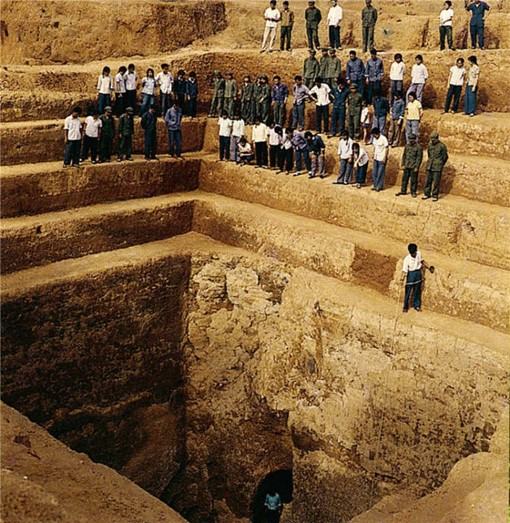
\includegraphics[width=\textwidth]{ConfucianismeTaoismeBouddhismeChinois/Images/tombelaozi.jpg}

    \label{fig:enter-label}
\end{marginfigure}

\paragraph{Biographie dans la tombe }On a trouvé la momie du Seigneur et sa biographie. Il aimé lire ces textes. Cinquantaine de textes et cartes géographiques,, philosophie, médecine, astronomie... 2 versions du Laozi.

 


 \begin{figure}[!h]
    \centering
        \sidecaption{Fragments de la version A du Laozi trouvés dans la tombe n° 3 de Mawangdui. Cette tombe, datant de 168 av. J.-C., appartenait à Li Xi, fils de la marquise de Dai.}
    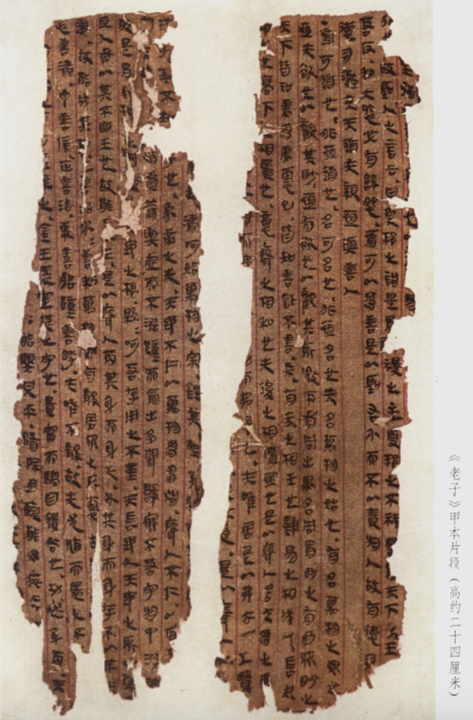
\includegraphics[width=0.5\textwidth]{ConfucianismeTaoismeBouddhismeChinois/Images/Laozitexte.png}

    \label{fig:enter-label}
\end{figure}
\paragraph{comparaison avec la version canonique} des différences, nuances, pas de divergences. Le style est plus dépouillé et clair que la version canonique : elle doit être plus proche du texte d'origine. 


 \subsection{version du Guodian}

 \paragraph{aussi au Sud de la Chine (fleuve Bleu)}

 \paragraph{Tombe}
Tombe n°1 de Guodian, datant du début du 4ème siècle av. J.-C., faisait partie d’un cimetière de l’ancienne capitale de la principauté de Chu, dans la province du Hubei actuelle. Elle a été découverte en 1993.

\paragraph{principauté de Chu} 
   
 
Les Etats indépendants avant l’unification de l’empire en 221 avant notre ère
  
\paragraph{lamelles de bambous} Manuscrits découverts dans la tombe n° 1 de Guodian. 

\paragraph{versions du Laozi}On a trouvé trois versions du Laozi. Ce qui est spécifique, c'est que ces trois versions ne se recoupent pas. L'ordre d'assemblage des textes n'est pas le mêmes entre versions. On peut donc choisir les chapitres qui nous intéresse. Au 4eme siècle av JC, il n'y a pas une version définitive ce qui permet de déduire que c'est uniquement au 3ème siècle qu'il y a une canonisation du texte.


\subsection{importance de l'Ecriture}

 
\paragraph{Taoisme : une doctrine, un culte}

\paragraph{l'Ecriture a une fonction sacrée} Dieu apparait et lui transmet les documents d'investiture. 

\paragraph{Arrivée du Bouddhisme} Pour faire face du Bouddhisme, le taoisme commence à produire des textes (4-5ème siècle de notre ère). Remettre au gout du jour les textes anciens. Ecrivent des codes moraux, instructions rituelles. Apocalypses et prophéties. 

\paragraph{influence bouddhique} bouche de la divinité (influence bouddhique).  Parsonnification du Tao. 

\paragraph{inventaire des textes taoistes au V après JC} Grâce à ces textes, reconnaissance par l'empereur et l'aristocratie. 



\subsection{La bureaucratie céleste}


\paragraph{role missionnaire du Taoisme} Tout un panthéon, construit au cours du temps. 

\paragraph{une bureaucratie céleste en extension} "2000 ans de bureaucratie" en Chine. 

\paragraph{personnification du Tapo} des dieux qui représentent les astres, les étoiles,...

\paragraph{au sommet, les 3 purs, manifestation du Tao} Il y a aussi des personnes réelles qui ont atteint l'immortalité, comme le Seigneur de Fengdu. 



 \begin{figure}[!h]
    \centering
        \sidecaption{À droite: « Le vénérable céleste du commencement originel »
Vers 1700 Musée Guimet; À gauche: « Le seigneur de Fengdu (les enfers taoïstes) et ses six ministres devenus immortels » Vers 1600
Musée Guimet}
    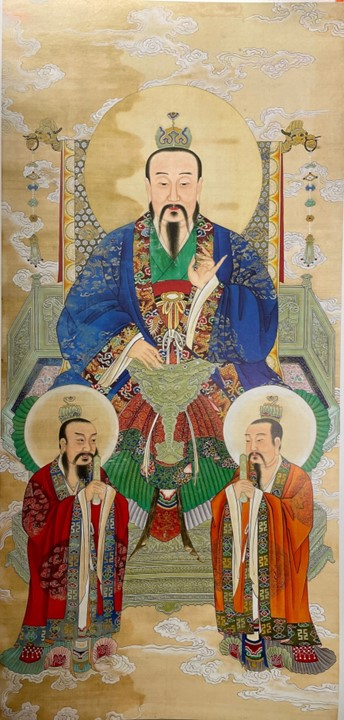
\includegraphics[width=0.4\textwidth]{ConfucianismeTaoismeBouddhismeChinois/Images/Levénérablecélesteducommencementoriginel.jpg}
    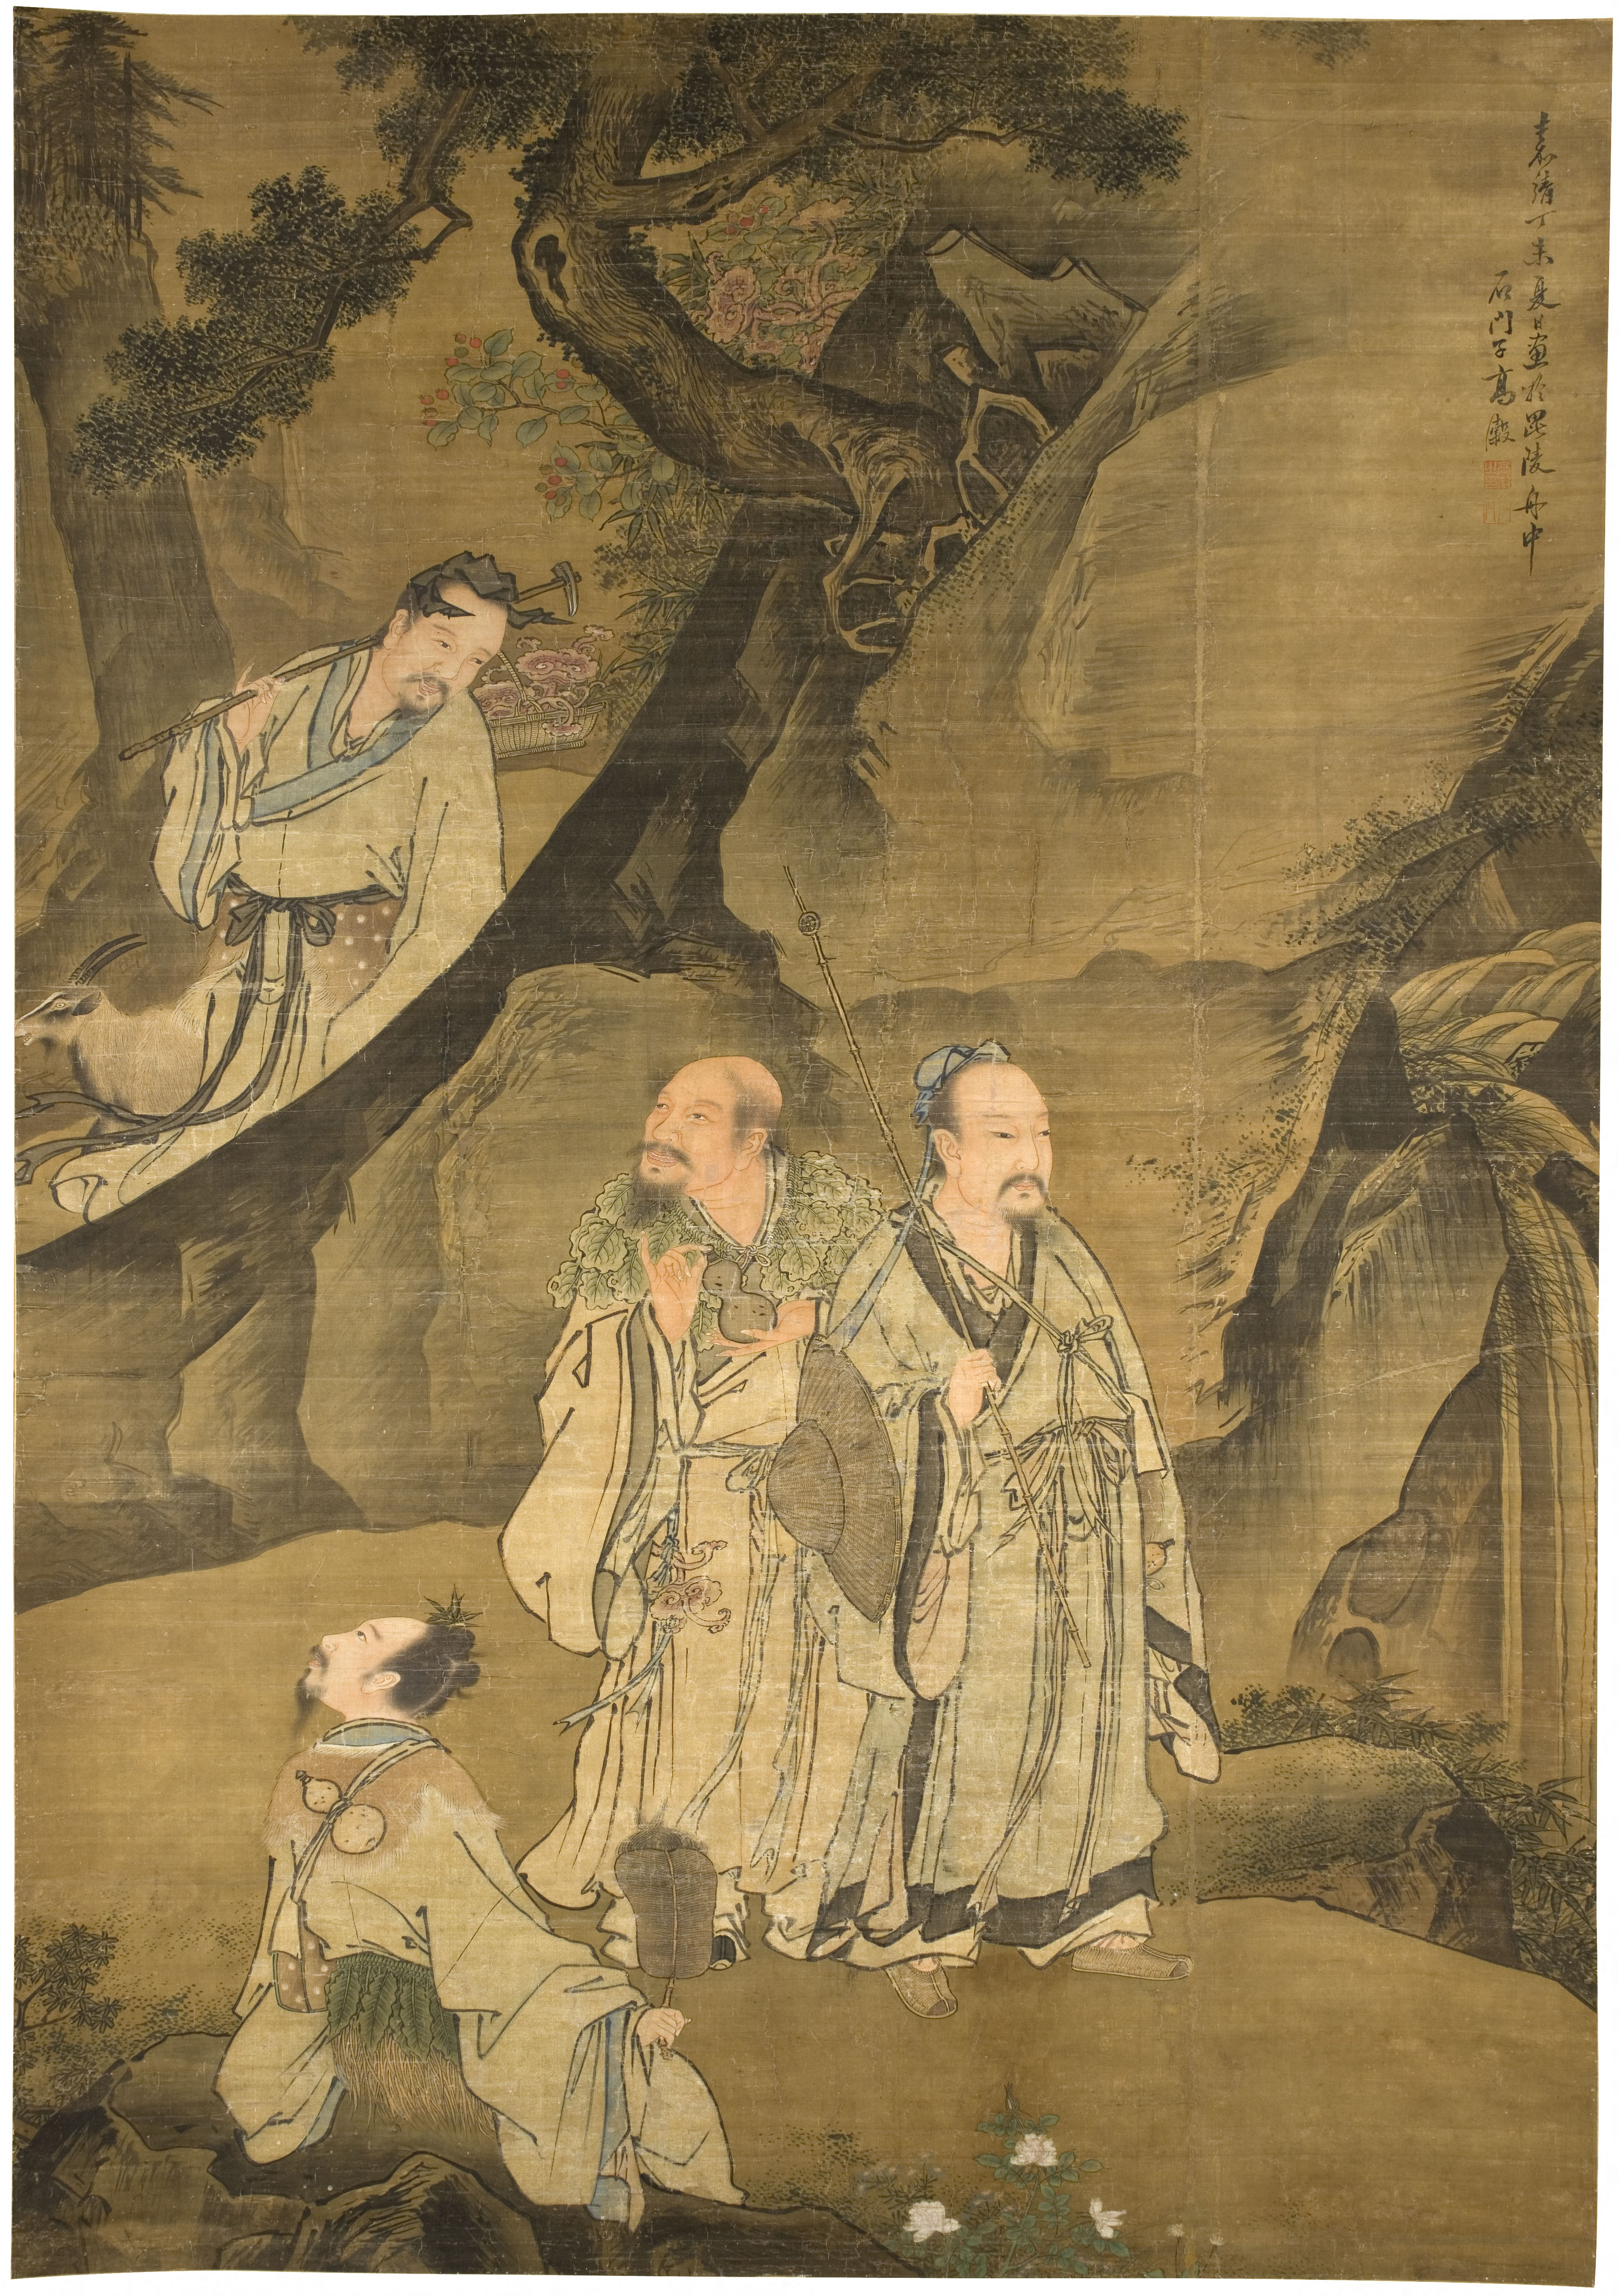
\includegraphics[width=0.54\textwidth]{ConfucianismeTaoismeBouddhismeChinois/Images/Immortels.jpg}
    \label{fig:enter-label}
\end{figure}





